\section{Evaluering}
\subsection{Test af Korrekthed}
Vi har som i \des løbende skrevet test før vi implementerede hver ny funktion i \code{RTP}-versionen.  Tabellen herunder viser testresultaterne for de test der er lavet specifikt for \code{RTP}-versionen.
\begin{longtable}{lr}
   	\toprule
    \mc{Test} & \mc{Resultat} \\
    \midrule
    \endfirsthead 
    \toprule
    \mc{Test} & \mc{Resultat} \\
    \midrule
    \endhead % slut efterfølgende headere
    \bottomrule
    \multicolumn{2}{r}{\textit{fortsættes}}
    \endfoot % slut footer
    \bottomrule
    \endlastfoot % slut sidste footer
test\_Alternation  & ok\\
test\_AlternationChoiseReader  & ok \\
test\_AlternationChoiseWriter  & ok \\
test\_AlternationExecuteReadDeadline  & ok\\
test\_AlternationExecuteSkipDeadline  & ok\\
test\_AlternationExecuteTimeoutDeadline  & ok \\
test\_AlternationExecuteWriteDeadline  & ok \\
test\_Alternationchoise1Deadline  & ok \\
test\_Alternationchoise2Deadline  & ok \\
test\_ChoisemultipleReader  & ok \\
test\_ChoisemultipleReader2  & ok \\
test\_ChoisemultipleWriter  & ok\\
test\_PoisonAndDeadline1  & ok\\
test\_PoisonAndDeadline2  & ok\\
test\_Reader\_Inheritance  & ok\\
test\_RetireAndDeadline  & ok\\
test\_Writer\_Inheritance  & ok\\
test\_channelpriority\_from\_low\_deadline  & ok\\
test\_channelpriority\_from\_low\_deadline2  & ok\\
test\_channelpriority\_from\_no\_deadline  & ok\\
test\_channelpriority\_from\_no\_deadline2  & ok\\
test\_readDeadline  &ok\\
test\_writeDeadline  & ok\\
test\_xreset\_inheritance  & ok\\
test\_xreset\_inheritance\_from\_two\_step  & FAIL\\
\end{longtable}


 Alle test med en undtagelse fungerer korrekt. Testen der fejler hedder test"_xreset"_inheritance"_from"_two"_step, og viser en situation hvor den samme proces får løftets sin prioritet to gange i træk, først med en høj prioritet, og efterfølgende med en mellemprioritet. Efterfølgende skal processen sænke sin prioritet, først til  mellemprioriteten og tilslut til sin originale prioritet. Her viser det sig vi har lavet en fejl i implementeringen, således at prioriteten ikke bliver nedsat til mellemprioriteten. \CRef{fig:priority-inheritance} viser prioriteten mens processen bliver op og nedprioriteret. Tiden har ikke tilladt os at løse problemet, men  kan løses ved at kræve at, når en proces opprioriteres gemmes hvilken proces der står bag, så når en proces ønsker at fjerne sin opprioritering fra andre processer er det kun sin egen  prioritet den fjerner.  
 
  
\begin{figure}
 \begin{center}
  
\includegraphics[scale=1]{images/priority-inheritance}
	\caption{Figuren viser hhv. forventet og faktisk prioritetsarvning. Der hvor den faktiske og forventede opførsel adskiller sig er forventet den fuldt optrukne streg, mens den stiplede streg er den faktiske opførsel.}
	\label{fig:priority-inheritance}
\end{center}
\end{figure}
  

\subsection{Slagterieksempel}

Først vil vi sammenligne de to udviklede versioner, for at se på deres fordele og ulemper, og til slut vi dette afsnit sammenholde de to versioner, med et  eksempel der er implementeret i RTP-versionen.

Helt generelt opnår man ved at basere koden på \pycsp et  netværk man nemt kan udvide hvis de fysiske rammer for slagteriet ændre sig. Viser det sig f.eks at kameraet holder den samlede produktivitet af netværket tilbage kan, slagteriet tilføjet endnu et kamera, og nemt udvide procesnetværket med endnu en kameraproces, som kan arbejde samtidigt med det første kamera. 

Forskellen i kode mellem greenlets og processes versionen består af en linje, som indikere hvilken version pycsp skal bruge. Resten af koden er identisk mellem de to versioner. En kørsel mellem de to versioner, som vist i \cref{tab:deadline-runs} viser dog at versionen har betydning for både andelen af grise der kan nå at blive bearbejdet, og hvor lang tid det tager i køre testen. Det skyldes at testen køres på en multikerne CPU hvor processerne dermed har mulighed for at køre parallelt. Greeneltsversionen derimod er begrændset til at kun en proces kan arbejde samtidigt hvorfor der er flere grise der ikke når at blive bearbejdetinden for sin deadline.

\begin{table}[htbp]
	\centering
	\begin{tabular}{lrr}
       	\toprule
        \mc{Version} & \mc{Succesrate (\%)} & \mc{Tidsforbrug (s)} \\
        \midrule
        Greenlets & 42 & 16,5\\
        Processes & 71 & 10,3\\
        \bottomrule
    \end{tabular}
	\caption[]{Gennemførslen af simulation hvor 100 grise bliver sendt igennem procesnetværket. }\\
	\label{tab:deadline-runs}
\end{table}

Forskellen på kørselstiderne skyldes at detektoren venter på at aflevere griseobjektet til kameraet, og først når objektet er afleveret venter processen. Om dette er en urealistisk opførsel vil kræve mere domæneviden. Kan detektoren f.eks styre transportbåndet der fører grisene hen til detektoren er det en rimelig antagelse, mens det er urealistisk hvis båndet kører uafhængigt at detektoren.

I \code{proceesses}-versionen findes der kun tre krævende processer og dermed kan der bearbejdes en gris i konvertering, analysen og Udvælgelse og udskæringsprocessen. Dette sikre at det er de tre  grise nærmest robotten der arbejdes på, men samtidigt betyder det at man maksimalt kan arbejde på tre grise samtidigt. Ved at øge antallet af grise man kan arbejde på, vil man få mere tid per gris til at foretage arbejdet. Man kan derfor tilføje flere konverterings og analyseprocesser, så man kunne fortage samtidig beregninger af flere grise. Dette vil dog øge antallet af processer der  kæmper mod hinanden for CPU-tid, og grisseobjekterne vil desuden kæmpe mod hinanden for at komme igennem netværket uden hensyn til hvilken gris der er nærmest robotten. Man risikere dermed en starvation situation hvor grise længere tilbage på transportbåndet overhaler grise længere fremme.


RTP udvidelsen bygger på \code{greenlets}-versionen, og derfor vil en genimplementation med RTP versionen lide under de samme begrænsninger som diskuteret i implementeringen i afsnit \cref{sec:deadline-exampel-implementation}. Der er dog også en række fordele som vi vil komme ind på her.

Ved implementering af slagterieksemplet i \code{RTP}-versionen, slipper de enkelte processer for at holde styr på tiden, og foretage sammenligningen om den enkelte gris deadline er overskredet. Når de modtager en gris sætter de deres egen deadline til grisens via funktionen \code{Set\_deadline}.  Hver proces skal til gengæld kunne håndtere at modtage en \code{DeadlineException}, som de i dette tilfælde blot kan håndteres ved at smide den nuværende gris væk, da den ikke længere er relevant, og  gå i gang med modtage en ny gris.

I \code{greenlets}-versionen kom vi ind på at processerne frivilligt skal afgive kontrollen, før robotten kan foretage udskæringen, men at der ikke findes en metode til midlertidigt at afgive kontrollen. Med \code{RTP}-versionen og funktionen \code{Release} har alle processer mulighed for med jævne mellemrum at afgive kontrollen så robotten rettidigt kan foretage selve udskæringen. Hermed skal vi ikke introducere en delt datastruktur, med de problemer den introducere og som vi snakkede om i afsnittet Barrierer på side \pageref{sec:barrierer}.
  
selvom det var nødvændigt at basere RTP på  \code{greenlets}-versionen, medfører det at  kun en proces kan være aktiv på samme tid. Dermed kan vi kun udnytte en processor, som  passer dårligt sammen med denne applikation.  Vi kan dog til dels afhælpe dette problem ved at udnytte at der i \code{greenlets}-versionen, findes en \code{IO}-dekorering. Denne dekorering placerer en funktion i en separat tråd, så flere funktioner kan køre samtidigt. Man skal her dog være opmærksom på at GIL'en stadig forhindre parallel udførsel. Eventuel parallel udførsel vil derfor kræve at koden i IO dekoreringen, kalder eksterne moduler som diskuteret i \cref{chap:csp}. 

Et problem ved at køre flere funktioner samtidigt og overlade kørslen til operativsystemets \sched, er at den ikke kender noget til vores interne planlægning. En brug af \code{IO}-dekorering og eksterne moduler til at sikre samtidighed skal derfor bruges med varsomhed og kun efter en analyse af den enkelte applikation, da samtidige processer på den samme processor lige som i \code{processes}-versionen vil kæmpe mod hinanden om processorresurser. 
 
for at sikre optimal arbejdsfordeling kan man udføre en række test, hvor man variere  antallet af processer. Med \code{RTP}-versionen kan man nemt ændrer på antallet af konvertering- og analyse-processer for at fintune applikationen og  udnytte den underliggende platform. \code{RTP}-versionen sikrer i modsætning til \code{processes}-versionen at netværket hele tiden har fokus på først at videresende grisene nærmest robotten. \CRef{fig:pig-network3} viser hvordan netværket kan se ud med flere konverterings og analyse processer. 

\begin{figure}
 \begin{center}
  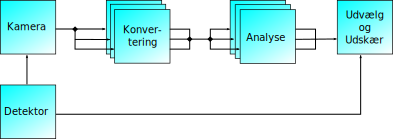
\includegraphics[scale=1]{images/pig-network3}
	\caption{Procesnetværk med flere konverteringsprocesser, og analyseprocesser}
	\label{fig:pig-network3}
\end{center}
\end{figure}
